\documentclass[12pt]{report}

% Paquetes LaTeX y estilos globales
\usepackage[utf8]{inputenc}
\usepackage{multicol}
\usepackage{xcolor}
\usepackage{subfigure}
\usepackage[spanish,es-tabla]{babel}
\usepackage[utf8]{inputenc}
\usepackage{graphicx}
\usepackage{titlesec}
\usepackage[bookmarks,breaklinks,colorlinks=true,allcolors=blue]{hyperref}
\usepackage{listings}
\usepackage{inconsolata}
\usepackage{float}
\usepackage{mathpazo} % Fuente Palatino
\usepackage[labelfont=bf]{caption}
\usepackage{comment}

\usepackage[square,numbers]{natbib}
\usepackage[nottoc,notlof,notlot]{tocbibind}  % Mete la bibliografía como capítulo en la TOC, los parámetros excluyen los otros índices de aparecer también
\usepackage{geometry}
\usepackage{amsmath}
\usepackage{parskip}
\usepackage[official]{eurosym}
\usepackage{todonotes}
\usepackage{csquotes}
\usepackage{tocbasic}  % Estilos de la TOC
\usepackage{hyperref}

% Formato del título de capítulos y secciones
\titleformat{\chapter}[block]{\normalfont\huge\bfseries}{\thechapter.}{.5em}{\Huge}[\vspace{2pt}{\titlerule[2pt]}]

\titlespacing*{\chapter}{0pt}{-19pt}{25pt}

\titleformat{\section}[block]{\normalfont\Large\bfseries}{\thesection.}{.5em}{\Large}

\titleformat{\part}[block]{\titlerule[2pt]\normalfont\Huge\bfseries\centering}{Parte \Roman{part}\\\vspace{15pt}}{0pt}{\Huge}[\vspace{2pt}{\titlerule[2pt]}] 

% Tamaños y estilos de elementos en la TOC
\DeclareTOCStyleEntry[
    linefill=\bfseries\TOCLineLeaderFill,
    beforeskip=12pt,
    entrynumberformat=\chapterprefixintoc,
    entryformat=\chaptertocformat,
    pagenumberformat=\chaptertocformat,
    dynnumwidth
]{tocline}{chapter}

\DeclareTOCStyleEntry[
    % linefill=\bfseries\TOCLineLeaderFill,
    beforeskip=30pt,
    entrynumberformat=\chapterprefixintoc,
    entryformat=\parttocformat,
    pagenumberformat=\partpagetocformat,
    numwidth=0pt
]{tocline}{part}

\newcommand\chaptertocformat[1]{\large{\textbf{#1}}}%
\newcommand\chapterprefixintoc[1]{#1}%
\newcommand\parttocformat[1]{\Large{\textbf{#1}}}%
\newcommand\partpagetocformat[1]{} % Don't print the page number for parts

% Alias para estilos de texto comunes
\newcommand{\negritas}[1]{\textbf{#1}}
\newcommand{\cursiva}[1]{\textit{#1}}
\newcommand{\codigo}[1]{\texttt{#1}}

% Formato del código fuente con lstlisting
\lstset{
  basicstyle=\ttfamily,
  breaklines=true,
}

% Márgenes
\geometry{
    a4paper,
    margin=2.75cm
}
\setlength{\marginparwidth}{2cm} 

\pagenumbering{arabic} % Números de página en arábico
 
% Limite de profundidad del índice
\setcounter{tocdepth}{2}

% Eliminar el guionado
\tolerance=1
\emergencystretch=\maxdimen
\hyphenpenalty=10000
\hbadness=10000

% Indentación de párrafos
\setlength{\parindent}{.75cm}

\renewcommand{\lstlistingname}{Extracto de código}
\renewcommand*{\lstlistlistingname}{Índice de extractos de código}

% Comandos para establecer variables
\newcommand{\setTitle}[1]{\def\tfgTitle {#1}}
\newcommand{\setAuthor}[1]{\def\tfgAuthors {#1}}
\newcommand{\setDegree}[1]{\def\tfgDegree {#1}}
\newcommand{\setSupervisor}[1]{\def\tfgSupervisor {#1}}
\newcommand{\setDepartment}[1]{\def\tfgDepartment {#1}}
\newcommand{\setMonth}[1]{\def\tfgMonth {#1}}
\newcommand{\setYear}[1]{\def\tfgYear {#1}}
\newcommand{\setDedication}[1]{\def\tfgDedication {#1}}

% Estilos para el código
% Configuración genérica
\definecolor{codegreen}{rgb}{0,0.6,0}
\definecolor{codegray}{rgb}{0.5,0.5,0.5}
\definecolor{codepurple}{rgb}{0.58,0,0.82}
\definecolor{editorOcher}{rgb}{0.8, 0.3, 0} % #FF7F00 -> rgb(239, 169, 0)
\definecolor{editorGreen}{rgb}{0, 0.5, 0} % #007C00 -> rgb(0, 124, 0)

\lstdefinestyle{listingstyle}{
    backgroundcolor=\color{white},  
    keywordstyle=\bfseries\color{blue},
    numberstyle=\tiny\color{codegray},
    stringstyle=\color{editorGreen},
    commentstyle=\color{codegray},
    basicstyle=\ttfamily\color{black},
    breakatwhitespace=false,         
    breaklines=true,                 
    captionpos=b,                    
    keepspaces=true,                 
    numbers=left,                    
    numbersep=5pt,                  
    showspaces=false,                
    showstringspaces=false,
    showtabs=false,                  
    tabsize=2,
    frame=tb,
    keywords=[2]{True,False},
    literate=%
*{0}{{{\color{editorOcher}0}}}1
{1}{{{\color{editorOcher}1}}}1
{2}{{{\color{editorOcher}2}}}1
{3}{{{\color{editorOcher}3}}}1
{4}{{{\color{editorOcher}4}}}1
{5}{{{\color{editorOcher}5}}}1
{6}{{{\color{editorOcher}6}}}1
{7}{{{\color{editorOcher}7}}}1
{8}{{{\color{editorOcher}8}}}1
{9}{{{\color{editorOcher}9}}}1,
}

\lstset{style=listingstyle}
\lstset{columns=fullflexible}

\lstdefinelanguage{css}{
  keywords={color,background-image:,margin,padding,font,weight,display,position,top,left,right,bottom,list,style,border,size,white,space,min,width, transition:, transform:, transition-property, transition-duration, transition-timing-function},	
  sensitive=true,
  morecomment=[l]{//},
  morecomment=[s]{/*}{*/},
  morestring=[b]',
  morestring=[b]",
  alsoletter={:},
  alsodigit={-}
}
% JavaScript
\lstdefinelanguage{javascript}{
  morekeywords={abstract, arguments, await, boolean, break, byte, case, catch, char, class, const, continue, debugger, default, delete, do, double, else, enum, eval, export, extends, false, final, finally, float, for, function, goto, if, implements, import, in, instanceof, int, interface, let, long, native, new, null, package, private, protected, public, return, short, static, super, switch, synchronized, this, throw, throws, transient, true, try, typeof, var, void, volatile, while, with, yield},
  morecomment=[s]{/*}{*/},
  morecomment=[l]//,
  morestring=[b]",
  morestring=[b]'
}

%Comentarios con todonotes
\newcommand{\Juanmi}[2][]{\todo[inline, color=green!30, caption={ToDo - Juanmi}, #1]{\begin{minipage}{\textwidth-4pt} #2\\ {\bf  -- Juanmi} \end{minipage}}}
\newcommand{\Juanlu}[2][]{\todo[inline, color=gray!20, caption={ToDo - Juanlu}, #1]{\begin{minipage}{\textwidth-4pt} #2 {\bf -- Juanlu}\end{minipage}}}


%%%%%%%%%%%%%%%%%%%%%%%%%%%%%%%%%%%%%%%%%%%%%%%%%%%%%%%%%%%%%%%%%%%%%%%%%%%%%%%%%%%%%

% Variables para la portada
\setTitle{CalendarUGR - Sistema de gestión personalizada de horarios académicos para la Universidad de Granada} 
\setAuthor{Juan Miguel Acosta Ortega} 
\setDegree{Grado en Ingeniería Informática} 
\setSupervisor{Juan Luis Jiménez Laredo} 
\setDepartment{Dpto. de Ingeniería de Computadores, Automática y Robótica}
\setMonth{junio} 
\setYear{2024/25} 

%%%%%%%%%%%%%%%%%%%%%%%%%%%%%%%%%%%%%%%%%%%%%%%%%%%%%%%%%%%%%%%%%%%%%%%%%%%%%%%%%%%%%

% Dedicatoria del trabajo
% Si no se desea incluir, comentar o borrar la línea siguiente para eliminar la página de dedicatoria
\setDedication{Aquí la dedicatoria del trabajo}

%%%%%%%%%%%%%%%%%%%%%%%%%%%%%%%%%%%%%%%%%%%%%%%%%%%%%%%%%%%%%%%%%%%%%%%%%%%%%%%%%%%%%

% Comienzo del documento
\begin{document}

    % Portada y secciones no numeradas
    \thispagestyle{empty} % Impide que se incluya número de página en la portada
\begin{center}

\vspace*{0.5cm}


\includegraphics[width=\textwidth]{figures/etsiit_ugr_logo.png}

\vspace*{1.5cm}
\begin{large}
TRABAJO FIN DE GRADO
\end{large}

\vspace*{0.1in}
\textbf{\huge \tfgTitle}

\vspace*{.2in}

{\large Realizado por}\\
\textbf{\Large \tfgAuthors}

\vspace*{3cm}

\textbf{Para la obtención del título de}\\
{\large \tfgDegree}

\vspace*{0.2in}

\textbf{Dirigido por}\\
{\large \tfgSupervisor}\\

\vspace*{0.2in}

\textbf{En el departamento de}\\
{\large \tfgDepartment}

\vspace*{.6in}
\textbf{\Large Convocatoria de \tfgMonth, curso \tfgYear}

\end{center}

% Dedicatoria
\ifdefined\tfgDedication
    \newpage
    \thispagestyle{empty}
    
    \vspace*{\fill}
    \begin{center}
    \textit{\tfgDedication}
    \end{center}
    \vspace*{\fill}
\fi

\clearpage\setcounter{page}{1} % Comienza a incluir números de página a partir de aquí
\pagenumbering{roman} % En números romanos
    \chapter*{Agradecimientos}

Este breve, pero sincero, apartado de agradecimientos comienza siendo un homenaje a todas las personas que alguna vez me han ayudado, apoyado o inspirado a lo largo de mi vida. Sin duda, cada uno de ellos ha dejado una huella en mi camino y ha contribuido a que hoy pueda presentar este trabajo.

Quiero expresar mi más profundo agradecimiento a mis padres, quienes siempre han estado a mi lado, brindándome su apoyo incondicional y enseñándome el valor del esfuerzo y la dedicación. Su amor y sacrificio han sido fundamentales en mi formación personal y académica.

A mi hermano, tropezar no significa caer, sino aprender a levantarse. El apoyo y la complicidad que hemos compartido a lo largo de los años han sido una fuente constante de motivación y alegría en mi vida. Gracias por todo.

A mis amigos, cada uno con sus propias historias, vivencias y enseñanzas, cada uno entrelazando su camino con el mío en épocas y distancias diferentes. Gracias por estar siempre a mi lado, por hacer que el viaje sea más llevadero y por compartir momentos inolvidables.

A mi novia, Laura, por su amor, paciencia y comprensión. Tu apoyo constante ha sido mi mayor motivación en cada paso que doy, tu presencia ilumina mis días y me impulsa a seguir adelante, incluso en los momentos más difíciles.

En último lugar, pero no menos importante, quiero agradecer a mi director de TFG, Juan Luis Jiménez Laredo, por su orientación, motivación, esfuerzo y dedicación durante todo el proceso. Su experiencia y conocimientos han sido invaluables para el desarrollo de este trabajo, y su apoyo constante me ha permitido superar los desafíos que se presentaron en el camino. Te has convertido sin duda en una fuente de inspiración y un modelo a seguir en mi vida académica y profesional. Gracias por tu confianza en mí y por guiarme en este proceso.

A todos ellos, mi más sincero agradecimiento. Este trabajo es un reflejo de su apoyo y confianza en mí, y espero que sea un digno homenaje a todo lo que han hecho por mí. Gracias por ser parte de mi vida y por ayudarme a alcanzar mis metas.
    \newpage
\begin{center}
    {\large \textbf{TempusUGR - Desarrollo de una Aplicación de Gestión de Horarios Universitarios Basada en Microservicios Interoperable con Servicios de Calendario Externos}}
    
    \vspace{0.3cm}
    {\normalsize Juan Miguel Acosta Ortega} 
    
    \vspace{0.3cm}
\end{center}

\vspace{0.5cm}

\textbf{Palabras clave:} Microservicios, Contenerización, Calendario Académico, Interoperabilidad, Backend, Autenticación

\vspace{0.5cm}

\textbf{Resumen:}

El presente Trabajo Fin de Grado aborda el diseño e implementación de un sistema backend para la gestión centralizada y la distribución dinámica del calendario académico de la Universidad de Granada. El proyecto nace de la necesidad de modernizar el acceso a la información académica, superando los desafíos de la dispersión de datos y la falta de integración con las herramientas de productividad digital actuales.

La solución se fundamenta en una arquitectura de microservicios contenerizados, seleccionada por su alta escalabilidad, resiliencia y facilidad de mantenimiento. El núcleo del sistema es una plataforma de suscripción que permite a estudiantes y profesores, previa autenticación segura con sus credenciales universitarias, generar calendarios personalizados. Cada usuario puede seleccionar los grupos de teoría y prácticas correspondientes a su matrícula o docencia, obteniendo una vista unificada y detallada que incluye asignaturas, aulas y profesorado.

Un pilar fundamental del proyecto es la interoperabilidad con servicios de calendario externos. El sistema permite a los usuarios exportar y sincronizar sus horarios personalizados con plataformas de amplio uso como Google Calendar. Esta funcionalidad garantiza el acceso a la información académica en tiempo real y desde cualquier dispositivo, eliminando la necesidad de consultas manuales y propensas a errores.

En definitiva, este trabajo no solo desarrolla una aplicación funcional, sino que establece una infraestructura tecnológica que optimiza la gestión del tiempo y mejora significativamente la experiencia de usuario para toda la comunidad de la UGR, promoviendo una gestión académica más eficiente, accesible y centralizada.

    \chapter*{Abstract}
This Final Degree Project addresses the design and implementation of a backend system for the centralized management and dynamic distribution of the academic calendar of the University of Granada (UGR). The project stems from the need to modernize access to academic information, overcoming the challenges of data dispersion and the lack of integration with current digital productivity tools.

The proposed solution is based on a containerized microservices architecture, selected for its high scalability, resilience, and ease of maintenance. The core of the system is a subscription platform that allows students and faculty, after secure authentication with their university credentials, to generate personalized calendars. Each user can select the lecture and practical groups corresponding to their enrollment or teaching assignments, obtaining a unified and detailed view that includes subjects, classrooms, and instructors.

A fundamental pillar of the project is interoperability with external calendar services. The system enables users to export and synchronize their personalized schedules with widely used platforms such as Google Calendar. This functionality ensures access to academic information in real-time and from any device, eliminating the need for manual and error-prone lookups.

In conclusion, this project not only develops a functional application but also establishes a technological infrastructure that optimizes time management and significantly enhances the user experience for the entire UGR community, promoting a more efficient, accessible, and centralized academic management.

\vspace{.5cm}

\textbf{Keywords:} Microservices, Containerization, Academic Calendar, Interoperability, Backend, Authentication
    \newpage \thispagestyle{empty} \mbox{} \newpage
\vspace{5cm}
\noindent\rule[-1ex]{\textwidth}{2pt}\\[4.5ex]

Yo, \textbf{Juan Miguel Acosta Ortega}, alumno de la titulación Grado en Ingeniería Informática de la \textbf{Escuela Técnica Superior
de Ingenierías Informática y de Telecomunicación de la Universidad de Granada}, con DNI 54313742R, autorizo la ubicación de la siguiente copia de mi Trabajo Fin de Grado en la biblioteca del centro para que pueda ser
consultada por las personas que lo deseen.

\vspace{6cm}

\noindent Fdo: Juan Miguel Acosta Ortega

\vspace{2cm}

\begin{flushright}
% Fecha actual
Granada, \today
\end{flushright}

\newpage \thispagestyle{empty} \mbox{} \newpage

\newpage
\vspace{5cm}
\noindent\rule[-1ex]{\textwidth}{2pt}\\[4.5ex]

D. \textbf{Juan Luis Jiménez Laredo}, Profesor del Área de Arquitectura y Tecnología de Computadores
del Departamento de Ingeniería de Computadores, Automática y Robótica de la Universidad de Granada.

\vspace{0.5cm}

\textbf{Informa:}

\vspace{0.5cm}

Que el presente trabajo, titulado \textit{\textbf{ TempusUGR - Desarrollo de una Aplicación de Gestión de Horarios Universitarios Basada en Microservicios Interoperable con Servicios de Calendario Externos }}, ha sido realizado bajo su supervisión por \textbf{Juan Miguel Acosta Ortega}, y autorizo la defensa de dicho trabajo ante el tribunal que corresponda.

\vspace{0.5cm}

Y para que conste, expide y firma el presente informe en Granada, \today.

\vspace{1cm}

\textbf{El director:} Juan Luis Jiménez Laredo

\newpage \thispagestyle{empty} \mbox{} \newpage
    
    % Índice del documento y de figuras
    \begingroup
        % Los enlaces son normalmente azules, pero en los índices se configuran a negro para que no aparezca todo azul
        \hypersetup{linkcolor=black}
        \tableofcontents
        \listoffigures
        \listoftables
        \lstlistoflistings
    \endgroup
    
    % Cambia el estilo de números de página de romanos a normal
    \clearpage\pagenumbering{arabic}
    
    % Capítulos del trabajo
    \chapter{Introducción}\label{cap:introduccion}

\section{Motivación}

La arquitectura de microservicios ha emergido como un paradigma fundamental en el desarrollo de sistemas complejos y escalables. Su enfoque modular y distribuido ofrece ventajas claras en términos de flexibilidad, mantenibilidad y despliegue independiente. Sin embargo, la implementación exitosa de una arquitectura de microservicios conlleva una serie de desafíos técnicos que resultan atractivos desde una perspectiva de aprendizaje y desarrollo profesional.

Este proyecto de fin de grado se presenta como una oportunidad perfecta para explorar de manera profunda los entresijos de esta arquitectura. Conceptos como la comunicación eficiente entre servicios (síncrona y asíncrona), la implementación de un API Gateway robusto para la gestión centralizada de peticiones, enrutamiento, seguridad ... , la aplicación de mecanismos de seguridad en un entorno distribuido, y las estrategias de balanceo de carga para garantizar la disponibilidad del sistema, representan áreas de gran interés práctico y teórico.

El desarrollo de un sistema de calendario personalizado para la Universidad de Granada, basado en una arquitectura de microservicios, permitirá no solo consolidar conocimientos teóricos, sino también enfrentarse a los retos inherentes a la construcción de un sistema distribuido real. La necesidad de diseñar APIs claras y bien definidas, gestionar la persistencia de datos en múltiples servicios, asegurar la consistencia y la tolerancia a fallos, y monitorizar el rendimiento del sistema en su conjunto, proporcionarán una experiencia de aprendizaje invaluable. En definitiva, este proyecto se concibe como un vehículo para comprender y aplicar de manera práctica los principios y las mejores prácticas asociadas a la arquitectura de microservicios, un campo con una alta demanda en la industria del desarrollo de software.

\section{Estructura de la memoria}

La estructura de la memoria se divide en los siguientes capítulos:

\begin{itemize}
    \item \textbf{Capítulo 1: Introducción.} En este capítulo se presenta la motivación del trabajo y la estructura de la memoria.
    \item \textbf{Capítulo 2: Descripción del problema.} En este capítulo se describe el problema que se va a resolver en el trabajo.
    \item \textbf{Capítulo 3: Estado del arte.} En este capítulo se presenta un resumen del estado del arte tanto en el ámbito de sistemas de gestión de horarios como en el ámbito de sistemas de información basados en web.
    \item \textbf{Capítulo 4: Especificación de requisitos.} En este capítulo se presentan las personas, escenarios, y los requisitos del sistema en forma de historias de usuario y requisitos funcionales, no funcionales, y de información.
    \item \textbf{Capítulo 5: Planificación.} En este capítulo se presenta la planificación temporal de trabajo, la metodología de desarrollo escogida y su implementación. Además se presenta un presupuesto del trabajo.
    \item \textbf{Capítulo 6: Diseño.} En este capítulo se presenta el diseño de la arquitectura de microservicios, de la API REST Implementada, de las bases de datos y del frontend desarrollado.
    \item \textbf{Capítulo 7: Implementación.} En este capítulo se presenta la implementación del sistema dividido en los sprints realizados.
    \item \textbf{Capítulo 8: Despliegue.} En este capítulo se presenta el despliegue del sistema en el servidor de la UGR con lo que todo ello conlleva ( gestión del servidor, SSL, HTTPS, dominio, etc.).
    \item \textbf{Capítulo 9: Conclusiones.} En este capítulo se presentan las conclusiones y trabajos futuros planteados.
    \item \textbf{Anexo A: Glosario.} En este anexo se presenta un glosario con las definiciones de términos técnicos utilizados a lo largo del trabajo.
\end{itemize}

    \chapter{Estado del arte}\label{cap:estado}

\section{Información de horarios académicos en la UGR}

La Universidad de Granada, al igual que muchas otras universidades descentraliza sus sedes, de modo que
cada una de ellas tiene su propio sistema de gestión de la información. En este sentido, las facultades cuentan
con una serie de sistemas de información propios que se encargan de la generación de horarios académicos,
asignación de aulas y profesores a los grupos tanto de teoría como de prácticas 
de las distintas titulaciones y asignaturas, etc. Y esta información a su vez se le facilita a la Universidad de Granada para la centralización de la información.
\newline\newline
Para acceder a la información de los horarios, los estudiantes y docentes pueden hacerlo de diferentes maneras:
\begin{itemize}
    \item A través de la página propia de su facultad. Poniéndo de ejemplo a la ETSIIT, debemos acceder a la página ``https://etsiit.ugr.es`` y buscar la información en la sección
          de ``Calendario de exámenes`` en caso de querer saber los días y rangos horarios de estos y visualizándolo con un pdf, o a ``Calendario académico y horarios`` y a ``Grado en Ingeniería Informática``
          en caso de querer saber los horarios de los diferentes grupos del grado, presentado todo ello en un pdf contenedor de alrededor de 40 tablas.
          \newline\newline
          De esta manera tendremos que buscar el año al que pertenece la asignatura de la que estamos matriculados y el grupo al que pertenecemos. De esta manera obtenemos su 
          franja horaria y aula, pero no profesor que imparte la asignatura.
          \newline\newline
          Sin embargo, el formato de las tablas cambia de un grado a otro, haciendo que el estudiante tenga que buscar la información de manera diferente en cada grado si está matriculado en más de uno, 
          y obteniendo información diferente. En el caso del grado de Administración y Dirección de Empresas por ejemplo, no se muestra el aula en la que se imparte la clase, pero sí las asignaturas bilingües, y
          los profesores que las imparten.
          \newline\newline
          Esta forma de visualización de horarios es muy poco eficiente, ya que el estudiante tiene que buscar la información de manera manual, es inconsistente entre grados, y no es accesible para personas con discapacidad visual.
          %% Comparación de horarios de diferentes grados ( 2 imágenes )
          %% Como se insertan dos imagenes en latex con un unico pie de foto -> 
          \newpage
            \begin{figure}[H]
                \centering
                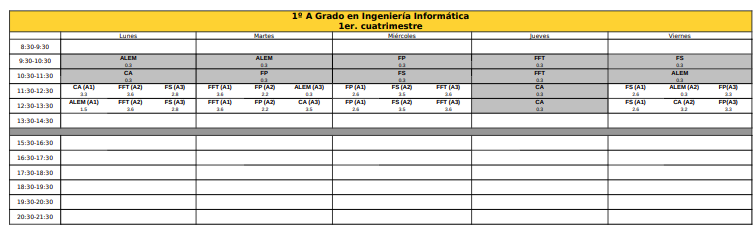
\includegraphics[width=0.8\textwidth]{figures/02_etsiit_horario.png}
                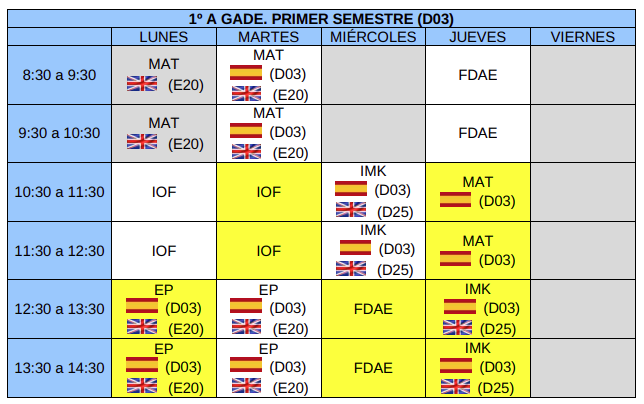
\includegraphics[width=0.8\textwidth]{figures/02_ade_horario.png}
                \caption{Comparación de horarios de diferentes grados: ETSIIT (arriba) y ADE (abajo).}
                \label{fig:horarios_comparacion}
            \end{figure}
          

    \item A través de la web ``https://grados.ugr.es/`` se puede buscar la información de los horarios de las asignaturas de los diferentes grados de la Universidad de Granada. Para ello debemos seleccionar rama de conocimiento, 
          grado, curso y asignatura. De esta manera obtenemos un horario semanal con las franjas horarias, aulas, profesores y fechas tanto de inicio como de fin. Este método nos proporcioan una interfaz estándar y más información, pero 
          también es más lento y tedioso para consultar por varias asignaturas o incluso grados.
    \item A través de las webs de cada departamento. Por ejemplo en la web de ``https://decsai.ugr.es/`` se puede consultar la información de las asignaturas o profesores de este.
          Ofrece información adicional como asignaturas que imparte ``x'' profesor y su horario de tutorías y docencia.
\end{itemize}

Además para acceder a la información de periodos de actividad docente, exámenes finales, periodos de evaluación de convocatorias ... se ha de acceder a la web de ``https://secretariageneral.ugr.es'' para consultar otro pdf.

En general la información de los horarios académicos de la Universidad de Granada es poco accesible, eficiente y consistente entre grados y facultades, lo que hace que el estudiante tenga que buscar la información de manera manual y tediosa.
Además no hay manera de consultar de manera sencilla un calendario personal que incluya tanto los horarios de las asignaturas como los exámenes y periodos de evaluación, entre otros.

\section{Comparación con otras instituciones}

\section{Acercamientos arquitectónicos}

\section{Tecnologías existentes}


    \chapter{Análisis del problema}\label{cap:analisis}

\section{Introducción}
En este capítulo explicaremos...

\section{Requisitos de información}
Los requisitos de información son...

\section{Requisitos funcionales}
Los requisitos funcionales son...

\section{Requisitos no funcionales}
Los requisitos no funcionales son...

\section{Conclusiones}
En este capítulo concluimos que...
    \input{sections/04_Diseño}
    \chapter{Implementación}\label{cap:implementacion}

\section{Introducción}
En este capítulo explicaremos...

\section {Herramientas}

\section{Conclusiones}
En este capítulo concluimos que...
    \chapter{Pruebas}\label{cap:pruebas}

\section{Introducción}
En este capítulo explicaremos...

\section{Conclusiones}
En este capítulo concluimos que...
    \chapter{Conclusiones y trabajos futuros}\label{cap:conclusiones}

\section{Evalución del proyecto}

\section{Dificultades y resolución}

\section{Mejoras posibles y trabajos futuros}


    % Bibliografía
    \bibliographystyle{unsrtnat}
    \bibliography{bibliografia.bib}

    % Anexos

    %% Anexo A : Glosario 
    \chapter*{Anexo A: Glosario}
\addcontentsline{toc}{chapter}{Anexo A: Glosario}

A continuación se presenta un glosario con las definiciones de términos técnicos utilizados a lo largo del trabajo:

\begin{description}
    \item [\hypertarget{scrum}{SCRUM}]: es un marco de trabajo ágil para el desarrollo de software. Se basa en la iteración y la colaboración entre los miembros del equipo de desarrollo.
    \item [\hypertarget{backlog}{Backlog}]: es una lista priorizada de tareas y requisitos que deben completarse en un proyecto. El backlog se utiliza para planificar el trabajo en cada sprint.
    \item [\hypertarget{lms}{LMS}]: es un sistema de gestión de aprendizaje. Se utiliza para administrar, documentar, rastrear, informar y entregar cursos de formación. Un ejemplo de LMS es Moodle, que es un sistema de gestión de aprendizaje de código abierto.
    \item [\hypertarget{docker}{Docker}]: es una plataforma de software que permite crear, desplegar y ejecutar aplicaciones en contenedores. Los contenedores son entornos ligeros y portátiles que permiten ejecutar aplicaciones de manera aislada del sistema operativo subyacente.
    \item [\hypertarget{microservicios}{Microservicios}]: es un estilo arquitectónico que estructura una aplicación como un conjunto de servicios pequeños y autónomos. Cada servicio se ejecuta en su propio proceso y se comunica con otros servicios a través de APIs.
    \item [\hypertarget{api}{API}]: es un conjunto de definiciones y protocolos que permiten la comunicación entre diferentes sistemas. Las APIs permiten que diferentes aplicaciones se comuniquen entre sí y compartan datos.
    \item [\hypertarget{backend}{Backend}]: es la parte de una aplicación que se encarga de la lógica de negocio y el acceso a los datos. El backend se ejecuta en un servidor y se comunica con el frontend a través de APIs.
    \item [\hypertarget{frontend}{Frontend}]: es la parte de una aplicación que se encarga de la interfaz de usuario y la interacción con el usuario. El frontend se ejecuta en el navegador del usuario y se comunica con el backend a través de APIs.
    \item [\hypertarget{ssl}{SSL}]: es un protocolo de seguridad que se utiliza para establecer una conexión segura entre un servidor y un cliente. SSL cifra los datos que se envían entre el servidor y el cliente, lo que protege la información sensible de ser interceptada por terceros.
    \item [\hypertarget{https}{HTTPS}]: es una versión segura de HTTP. HTTPS utiliza SSL para cifrar los datos que se envían entre el servidor y el cliente, lo que protege la información sensible de ser interceptada por terceros.
    \item [\hypertarget{ui}{UI}]: es la interfaz de usuario. Se refiere a la parte de una aplicación con la que el usuario interactúa. La UI incluye elementos como botones, menús y formularios.
    \item [\hypertarget{ux}{UX}]: es la experiencia del usuario. Se refiere a la forma en que un usuario interactúa con una aplicación y cómo se siente al hacerlo. La UX incluye aspectos como la usabilidad, la accesibilidad y la satisfacción del usuario.
    \item [\hypertarget{jwt}{JWT}]: es un estándar abierto que define un formato compacto y autónomo para transmitir información de forma segura entre partes como un objeto JSON. Esta información puede ser verificada y confiable porque está firmada digitalmente.
    \item [\hypertarget{sso}{SSO}]: es un proceso de autenticación que permite a un usuario acceder a múltiples aplicaciones con una sola sesión de inicio de sesión. SSO simplifica la gestión de credenciales y mejora la experiencia del usuario al reducir la necesidad de recordar múltiples contraseñas.
    \item [\hypertarget{rest}{REST}]: es un estilo arquitectónico para diseñar servicios web. REST se basa en el uso de HTTP y utiliza los métodos HTTP (GET, POST, PUT, DELETE) para realizar operaciones sobre recursos.
    \item [\hypertarget{graphql}{GraphQL}]: es un lenguaje de consulta para APIs y un entorno de ejecución para ejecutar esas consultas con los datos existentes. GraphQL permite a los clientes solicitar solo los datos que necesitan, lo que reduce la cantidad de datos transferidos entre el cliente y el servidor.
    \item [\hypertarget{grpc}{gRPC}]: es un marco de trabajo de código abierto que permite la comunicación entre aplicaciones distribuidas. gRPC utiliza HTTP/2 para la comunicación y Protocol Buffers como formato de serialización de datos.
\end{description}

\endinput
    %% Anexo B : Sprint Backlogs 
    \chapter*{Anexo B: Sprint Backlogs}
\addcontentsline{toc}{chapter}{Anexo B: Sprint Backlogs}
        

% Fin del documento
\end{document}
